% Level ceiling (grade 6): density handled as "mass of one cubic
% centimetre" via proportionality tables and division; the literal
% formula rho = m/V waits for grade 7 (literal expressions, math g7).
\chapter{Massa Jenis: Mengapa Benda Terapung}\label{ch:g6:density-floating}

Pada tahun pertamamu, sekeping koin mungil \omterm{def:g1:floating-and-sinking:words}{tenggelam} sementara
sebatang kayu besar \omterm{def:g1:floating-and-sinking:words}{terapung}, dan kita berjanji bahwa ``mengapa''-nya
adalah harta pelajaran ini. Kamu sudah pantas mendapatkannya. Kuncinya
ditempa lewat dua bab --- \omterm{def:g3:measuring-mass:mass}{massa} untuk zatnya, \omterm{def:g6:mass-and-volume:volume}{volume} untuk ruangnya
--- dan hari ini keduanya berputar bersama di dalam kuncinya.

\section{Massa satu sentimeter kubik}

\begin{example}[Akhirnya perbandingan yang adil]\label{ex:g6:density-floating:fair}
Membandingkan sebatang kayu utuh dengan sekeping koin utuh tidak
pernah adil: ukurannya berbeda, bentuknya berbeda. Pertandingan yang
adil mengambil \emph{\omterm{def:g6:mass-and-volume:volume}{volume} yang sama}: satu \omterm{def:g6:mass-and-volume:volume}{sentimeter kubik} dari
tiap peserta. Satu \unit{cm^3} air bermassa \qty{1}{g}. Satu
\unit{cm^3} kayu ek: kira-kira \qty{0.6}{g}. Batu: kira-kira
\qty{2.5}{g}. Besi: \qty{7.9}{g}. Ruang yang sama, zat yang jauh
berbeda --- inilah bilangan yang ditunggu permainan \omterm{def:g1:floating-and-sinking:words}{terapung} itu.
\end{example}

\begin{definition}[Massa jenis]\label{def:g6:density-floating:density}
Yang disebut \emph{massa jenis}\index{massa jenis} sebuah zat adalah
\omterm{def:g3:measuring-mass:mass}{massa} satu \omterm{def:g6:mass-and-volume:volume}{sentimeter kubik} zat itu, dalam \omterm{def:g3:measuring-mass:units}{gram}. \omterm{def:g3:measuring-mass:mass}{Massa} jenis air
adalah \qty{1}{g} tiap \unit{cm^3}; kayu ek kira-kira $0.6$; besi
$7.9$. Untuk mencari \omterm{def:g3:measuring-mass:mass}{massa} jenis, tidak diperlukan alat baru: ukurlah
\omterm{def:g3:measuring-mass:mass}{massa} sebuah cuplikan dan \omterm{def:g6:mass-and-volume:volume}{volumenya}, lalu bagilah --- bagikan \omterm{def:g3:measuring-mass:units}{gramnya}
sama rata di antara \omterm{def:g6:mass-and-volume:volume}{sentimeter kubiknya}, dan jawabannya adalah jatah
tiap \omterm{def:g6:mass-and-volume:volume}{sentimeter kubiknya}.
\end{definition}

\begin{omfigure}
\begin{tikzpicture}[scale=0.85]
  \foreach \x/\name/\m/\c in {0.9/gabus/0.2/omMeth,
      3.0/{kayu ek}/0.6/omMeth, 5.1/air/1.0/omDef,
      7.2/batu/2.5/omExo, 9.3/besi/7.9/omThm} {
    \draw[thick, fill=\c, fill opacity=0.4]
      (\x,0.6) rectangle ++(1.0,1.0);
    \node[above, font=\footnotesize] at (\x+0.5,1.65) {\name};
    \node[below, font=\footnotesize] at (\x+0.5,0.5)
      {$\m$ g};
  }
  \node[below, font=\small] at (5.6,-0.15)
    {lima kubus yang sama, tiap satu sentimeter kubik --- lima massa};
\end{tikzpicture}

{\small Pertandingan yang adil: ruang yang sama untuk semuanya, dan
tiap zat menunjukkan \omterm{def:g3:measuring-mass:mass}{massa} tanda tangannya.}
\end{omfigure}

\begin{proposition}[Massa jenis adalah tanda tangan]\label{prop:g6:density-floating:signature}
\omterm{def:g6:density-floating:density}{Massa jenis} sebuah zat murni sama untuk setiap kepingnya, besar maupun
kecil: sepotong serpih kayu ek dan sebatang balok utuh sama-sama
membawa kira-kira \qty{0.6}{g} pada tiap \omterm{def:g6:mass-and-volume:volume}{sentimeter kubiknya}. Karena
itu \omterm{def:g6:density-floating:density}{massa jenis} mengenali zat, seperti yang dilakukan \omterm{def:g4:changes-of-state:melting-point}{titik lebur}:
ukurlah \omterm{def:g3:measuring-mass:mass}{massa} dan \omterm{def:g6:mass-and-volume:volume}{volume} sebuah benda misterius, bagilah, lalu
bandingkan dengan tabelnya --- zatnya sering mengaku di tempat.
\end{proposition}

\begin{method}[Mengukur massa jenis]\label{met:g6:density-floating:measure}
Untuk sebutir kerikil --- atau sebuah mahkota:
\begin{enumerate}
  \item ukurlah \omterm{def:g3:measuring-mass:mass}{massanya} dengan \omterm{def:g3:levers-and-scales:scale}{neraca}: misalkan \qty{75}{g};
  \item ukurlah \omterm{def:g6:mass-and-volume:volume}{volumenya} dengan cara kenaikan air: misalkan
        \qty{30}{cm^3};
  \item bagilah \omterm{def:g3:measuring-mass:units}{gramnya} dengan \omterm{def:g6:mass-and-volume:volume}{sentimeter kubiknya}: $75 \div 30 =
        2.5$ --- tiap \omterm{def:g6:mass-and-volume:volume}{sentimeter kubiknya} membawa \qty{2.5}{g};
  \item lihatlah tabelnya: \omterm{def:g6:density-floating:density}{massa jenis} $2.5$ --- kerikil kita adalah
        batu biasa.
\end{enumerate}
\end{method}

\section{Aturan terapung}

\begin{proposition}[Mengapa benda terapung]\label{prop:g6:density-floating:rule}
Sebuah benda \omterm{def:g1:floating-and-sinking:words}{terapung} di air kalau \omterm{def:g3:measuring-mass:mass}{massa} jenisnya \emph{kurang}
daripada \omterm{def:g6:density-floating:density}{massa jenis} air --- kurang daripada \qty{1}{g} tiap
\omterm{def:g6:mass-and-volume:volume}{sentimeter kubik} --- dan \omterm{def:g1:floating-and-sinking:words}{tenggelam} kalau \omterm{def:g3:measuring-mass:mass}{massa} jenisnya lebih besar.
Airnya, boleh dikatakan, membandingkan si penyusup dengan dirinya
sendiri, ruang demi ruang: yang lebih ringan daripadaku tiap ruang
menumpang di atas; yang lebih berat tiap ruang turun ke bawah. Aturan
yang sama berlaku bagi \omterm{def:g3:solids-liquids-gases:liquid}{zat cair} mana pun, masing-masing dengan \omterm{def:g3:measuring-mass:mass}{massa}
jenisnya sendiri sebagai wasit.
\end{proposition}

\begin{omfigure}
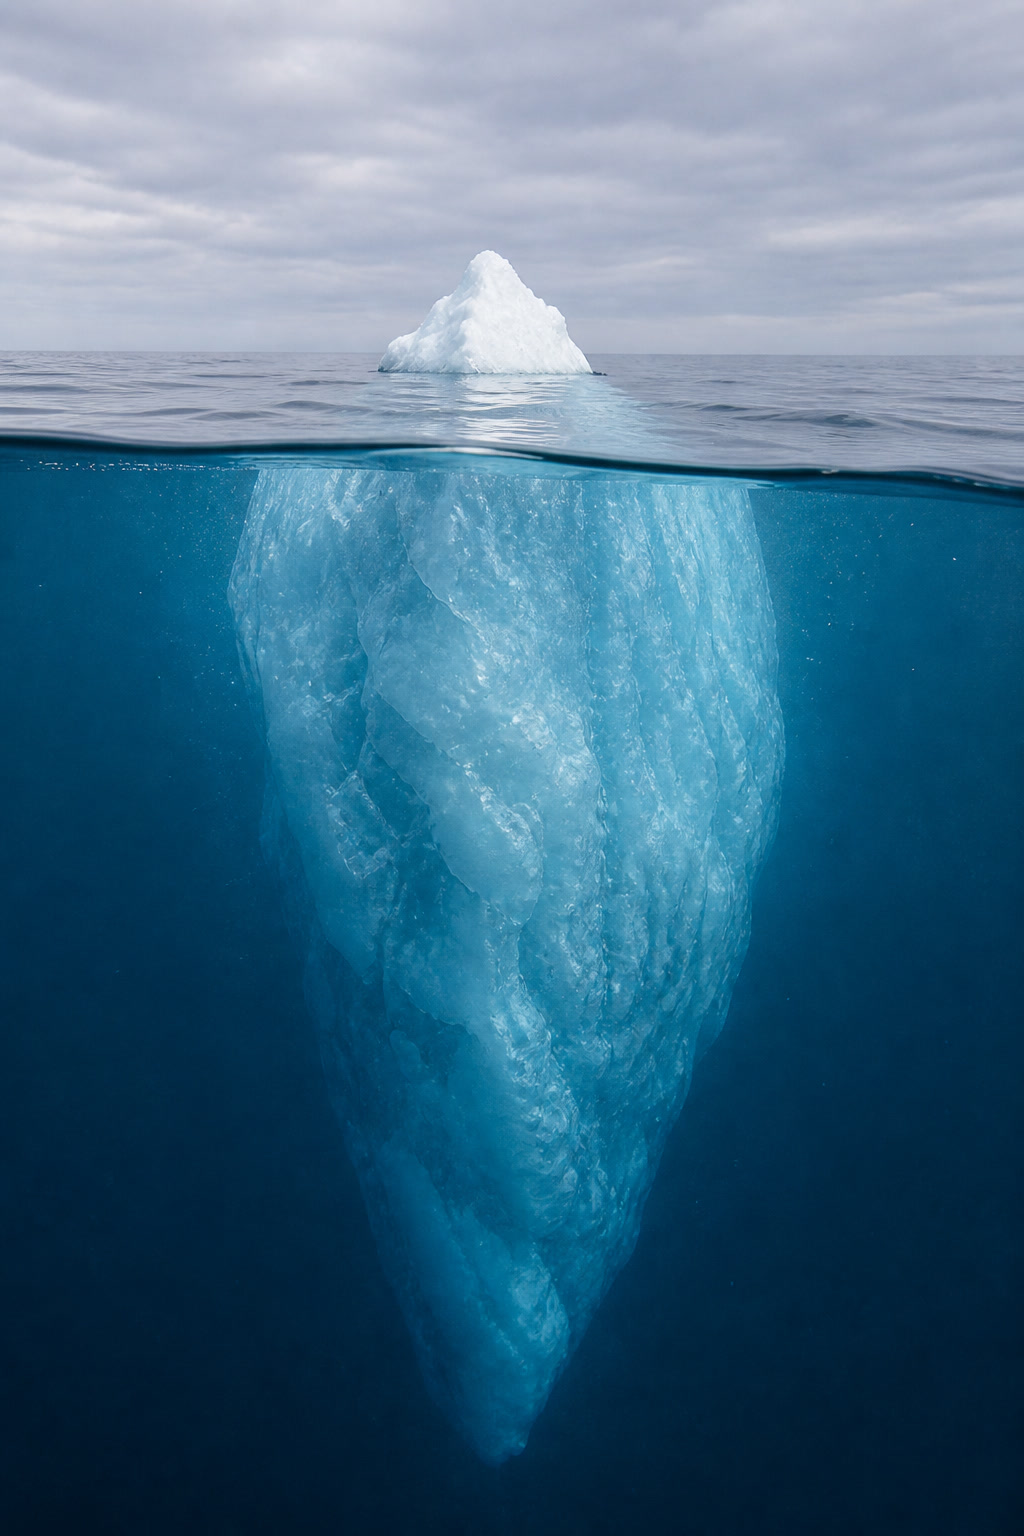
\includegraphics[width=0.4\linewidth]{images/book1/ai/g6-density-iceberg.jpg}

{\small \omterm{def:g6:density-floating:density}{Massa jenis} es hanya sedikit lebih kecil daripada \omterm{def:g6:density-floating:density}{massa jenis} air --- sehingga gunung es \omterm{def:g1:floating-and-sinking:words}{terapung} dalam-dalam, menyembunyikan sebagian besar tubuhnya di bawah garis air.}
\end{omfigure}

\begin{example}[Enam tahun teka-teki, terselesaikan]\label{ex:g6:density-floating:settled}
Batang kayu ($0.6$): \omterm{def:g1:floating-and-sinking:words}{terapung}, sebesar apa pun --- tiap \omterm{def:g6:mass-and-volume:volume}{sentimeter
kubiknya} menawar lebih rendah daripada air. Koinnya (perunggu, dekat
$9$): \omterm{def:g1:floating-and-sinking:words}{tenggelam}, sekecil apa pun. Bebek plastik, gabus, pensil: di
bawah $1$, semuanya \omterm{def:g1:floating-and-sinking:words}{terapung}. Es, pada $0.9$ --- \omterm{def:g3:solids-liquids-gases:solid}{zat padat} air sendiri
yang menggembung --- \omterm{def:g1:floating-and-sinking:words}{terapung} di atas \omterm{def:g3:solids-liquids-gases:liquid}{zat cairnya} sendiri dengan
selisih setipis rambut, dan itulah sebabnya kolam mengenakan tutup dan
gunung es berlayar. Dan perahu plastisinnya? Ketika dibentuk sebagai
mangkuk, bungkusan \emph{perahu-beserta-udara} memuat banyak \omterm{def:g2:air-around-us:air}{udara}
tiap ruang: \omterm{def:g6:density-floating:density}{massa jenis} bungkusan itu turun di bawah $1$, dan di
pelabuhan tipuan yang sama meluncurkan kapal baja sepuluh ribu ton.
\end{example}

\begin{omfigure}
\begin{tikzpicture}[scale=0.85]
  \draw[thick] (0.8,0) -- (0.8,3.4) (4.0,0) -- (4.0,3.4)
    (0.8,0) -- (4.0,0);
  \fill[omMeth, opacity=0.35] (0.8,2.2) rectangle (4.0,3.0);
  \node[font=\footnotesize] at (2.4,2.6) {minyak: $0.9$};
  \fill[omDef, opacity=0.3] (0.8,1.1) rectangle (4.0,2.2);
  \node[font=\footnotesize] at (2.4,1.65) {air: $1.0$};
  \fill[omThm, opacity=0.3] (0.8,0.05) rectangle (4.0,1.1);
  \node[font=\footnotesize] at (2.4,0.55) {madu: $1.4$};
  \node[below, font=\small] at (2.4,-0.3)
    {menara zat cair: yang paling padat di dasarnya};
  \draw[thick] (7.2,0) -- (7.2,3.4) (11.0,0) -- (11.0,3.4)
    (7.2,0) -- (11.0,0);
  \fill[omDef, opacity=0.3] (7.2,0.05) rectangle (11.0,2.6);
  \draw[thick, fill=white]
    (8.3,2.35) -- (9.9,2.35) -- (9.6,2.95) -- (8.6,2.95) -- cycle;
  \draw[thick, fill=white, fill opacity=0.7]
    (8.0,2.35) -- (10.2,2.35) -- (9.5,1.0) -- (8.7,1.0) -- cycle;
  \node[font=\footnotesize] at (9.1,1.85) {es: $0.9$};
  \node[below, font=\small] at (9.1,-0.3)
    {gunung es: sembilan persepuluh di bawah garis air};
\end{tikzpicture}

{\small Tulisan tangan \omterm{def:g6:density-floating:density}{massa jenis}: \omterm{def:g3:solids-liquids-gases:liquid}{zat cair} bertumpuk dengan yang
terpadat di bawah, dan es pada $0.9$ menumpang dengan hanya
sepersepuluh dirinya di atas air.}
\end{omfigure}

\begin{example}[Menara zat cair]\label{ex:g6:density-floating:tower}
Tuangkan madu, lalu air yang diwarnai tinta, lalu minyak pelan-pelan
menyusuri dinding gelas yang tinggi: tiga lapisan, madu ($1.4$) di
dasarnya, minyak ($0.9$) di puncaknya, yang menolak mencampur
pangkatnya. Jatuhkan tamu ke dalamnya: sebutir anggur ($1.05$)
\omterm{def:g1:floating-and-sinking:words}{tenggelam} menembus minyaknya, \omterm{def:g1:floating-and-sinking:words}{tenggelam} menembus airnya, lalu
bertumpu di atas madunya --- lebih padat daripada dua lantai, lebih
ringan daripada lantai yang ketiga. Menara itu adalah aturan \omterm{def:g1:floating-and-sinking:words}{terapung}
yang dipentaskan sebagai teater.
\end{example}

\begin{remark}[Membaca gunung es]\label{rem:g6:density-floating:iceberg}
Angka $0.9$ milik es melawan $1.0$ milik air melakukan lebih daripada
sekadar mengapungkan gunung esnya: ia menetapkan garis airnya.
Sembilan persepuluh tubuh sebuah gunung es menumpang \emph{di bawah}
permukaannya --- \omterm{def:g3:measuring-mass:mass}{massa} tersembunyi yang termasyhur, yang pernah
menenggelamkan kapal yang megah. \emph{Mengapa} tepatnya pecahan yang
di bawah itu cocok dengan perbandingan \omterm{def:g3:measuring-mass:mass}{massa} jenisnya adalah hukum
indah milik ilmuwan bak mandi zaman kuno itu sendiri, yang dibuktikan
dengan jujur di jilid Sekolah Menengah; tabel \omterm{def:g3:measuring-mass:mass}{massa} jenisnya sudah
membisikkan jawabannya.
\end{remark}

\section{Mahkotanya, akhirnya}

\begin{example}[Archimedes menutup perkaranya]\label{ex:g6:density-floating:crown}
Sekarang selesaikan kisah yang dimulai dua bab lalu. \omterm{def:g3:measuring-mass:mass}{Massa} mahkotanya:
mudah, \omterm{def:g3:levers-and-scales:scale}{neraca} memberikannya. \omterm{def:g6:mass-and-volume:volume}{Volumenya}: mustahil bagi mahakarya yang
bergumpal --- sampai pelajaran bak mandi memberikan cara kenaikan air.
\omterm{def:g3:measuring-mass:mass}{Massa} dibagi \omterm{def:g6:mass-and-volume:volume}{volume}: itulah \emph{\omterm{def:g6:density-floating:density}{massa jenis}} mahkotanya --- dan
\omterm{def:g6:density-floating:density}{massa jenis} adalah tanda tangan. Emas murni menandatangani $19.3$;
perak menandatangani $10.5$; campuran rahasia menandatangani sesuatu
di antaranya. Konon mahkota si pandai emas mengaku dengan \omterm{def:g6:density-floating:density}{massa jenis}
yang jauh di bawah \omterm{def:g6:density-floating:density}{massa jenis} emas, dan kecurangannya terbongkar
tanpa satu goresan pun pada mahkotanya. Soal akhir pekan menyerahkan
bilangannya kepadamu.
\end{example}

\section{Latihan}

\begin{exercise}[$\star$]\label{exo:g6:density-floating:1}
Apa itu \omterm{def:g6:density-floating:density}{massa jenis} sebuah zat? Sebutkan \omterm{def:g6:density-floating:density}{massa jenis} air, lalu
nyatakan aturan \omterm{def:g1:floating-and-sinking:words}{terapungnya}.
\end{exercise}

\begin{exercise}[$\star$]\label{exo:g6:density-floating:2}
Ramalkan \omterm{def:g1:floating-and-sinking:words}{terapung} atau \omterm{def:g1:floating-and-sinking:words}{tenggelam} di air: kayu ek ($0.6$); \ batu
($2.5$); \ gabus ($0.2$); \ besi ($7.9$); \ es ($0.9$).
\end{exercise}

\begin{exercise}[$\star$]\label{exo:g6:density-floating:3}
Sebuah balok bermassa \qty{120}{g} dan bervolume \qty{80}{cm^3}.
Carilah \omterm{def:g3:measuring-mass:mass}{massa} jenisnya. \omterm{def:g1:floating-and-sinking:words}{Terapung} atau \omterm{def:g1:floating-and-sinking:words}{tenggelam}?
\end{exercise}

\begin{exercise}[$\star$]\label{exo:g6:density-floating:4}
Sebuah gumpalan misterius: \omterm{def:g3:measuring-mass:mass}{massanya} \qty{158}{g}, kenaikan pada gelas
ukurnya \qty{20}{cm^3}. Berapa \omterm{def:g3:measuring-mass:mass}{massa} jenisnya --- dan, dari bilangan
dalam bab ini, kira-kira zat apa dia?
\end{exercise}

\begin{exercise}[$\star$]\label{exo:g6:density-floating:5}
Mengapa \omterm{def:g6:density-floating:density}{massa jenis} sepotong serpih kayu ek sama dengan \omterm{def:g6:density-floating:density}{massa jenis}
sebatang balok kayu ek yang utuh? Sifat ini berguna untuk apa?
\end{exercise}

\begin{exercise}[$\star$]\label{exo:g6:density-floating:6}
Pada menara \omterm{def:g3:solids-liquids-gases:liquid}{zat cair}, mengapa madu duduk di dasarnya dan minyak di
puncaknya? Di mana sebutir anggur bermassa jenis $1.05$ berhenti?
\end{exercise}

\begin{exercise}[$\star$]\label{exo:g6:density-floating:7}
Es \omterm{def:g1:floating-and-sinking:words}{terapung} di atas air --- mengapa hal ini aneh bagi sebuah \omterm{def:g3:solids-liquids-gases:solid}{zat
padat}, dan proposisi lama yang mana tentang air yang \omterm{def:g2:ice-water-steam:meltfreeze}{membeku} yang
menjelaskan angka $0.9$ itu?
\end{exercise}

\begin{exercise}[$\star$]\label{exo:g6:density-floating:8}
Batang kayu yang besar dan koin yang kecil pada tahun pertamamu:
berikan jawaban terakhirnya yang lengkap, dengan bilangan dari bab
ini.
\end{exercise}

\begin{exercise}[$\star\star$]\label{exo:g6:density-floating:9}
Satu \omterm{def:g6:mass-and-volume:volume}{liter} sebuah \omterm{def:g3:solids-liquids-gases:liquid}{zat cair} bermassa \qty{800}{g}. Berapa \omterm{def:g3:measuring-mass:mass}{massa}
jenisnya dalam \omterm{def:g3:measuring-mass:units}{gram} tiap \omterm{def:g6:mass-and-volume:volume}{sentimeter kubik}? Akankah sebongkah es
($0.9$) \omterm{def:g1:floating-and-sinking:words}{terapung} atau \omterm{def:g1:floating-and-sinking:words}{tenggelam} di dalamnya?
\end{exercise}

\begin{exercise}[$\star\star$]\label{exo:g6:density-floating:10}
Baja menandatangani $7.9$, namun kapal baja \omterm{def:g1:floating-and-sinking:words}{terapung}. Selesaikan
kejanggalannya dengan gagasan bungkusan pada
\cref{ex:g6:density-floating:settled} --- apa saja yang termasuk
bungkusan kapalnya selain baja, dan berapa \omterm{def:g6:density-floating:density}{massa jenis}
keseluruhannya harus? Kapan kapal yang berlubang berhenti memenuhi
aturannya?
\end{exercise}

\begin{exercise}[$\star\star$]\label{exo:g6:density-floating:11}
Air laut sedikit lebih padat daripada air tawar --- kira-kira $1.03$.
Jelaskan mengapa perenang \omterm{def:g1:floating-and-sinking:words}{terapung} jelas lebih baik di laut, lalu
ramalkan apa yang terjadi pada garis air sebuah kapal ketika ia
berlayar dari laut yang asin masuk ke sungai yang tawar.
\end{exercise}

\begin{exercise}[$\star\star\star$]\label{exo:g6:density-floating:12}
Sebuah bola logam berongga \omterm{def:g1:floating-and-sinking:words}{terapung} tepat setengah terbenam di air.
Nalarkan berapa \omterm{def:g6:density-floating:density}{massa jenis} \emph{seluruh bungkusan bolanya}
(cangkang logam ditambah \omterm{def:g2:air-around-us:air}{udara} di dalamnya). Lalu beralasanlah ke arah
mana ia bergerak kalau air perlahan merembes masuk, dan pada saat apa
ia mulai \omterm{def:g1:floating-and-sinking:words}{tenggelam} --- aturan dan bungkusan, bekerja bersama.
\end{exercise}

\section{Soal: Mahkota Sang Raja}

\begin{problem}[{Soal akhir pekan --- perkara mahkota sang raja,
dibuka kembali dengan alat ukurmu; pengadilan si pandai emas,
dipecahkan dengan pembagian}]\label{pb:g6:density-floating:1}
Bukalah kembali perkara kecurangan paling termasyhur zaman kuno dengan
bilangan zaman sekarang. Tanda tangannya: emas $19.3$, perak $10.5$
(\omterm{def:g3:measuring-mass:units}{gram} tiap \omterm{def:g6:mass-and-volume:volume}{sentimeter kubik}).

\medskip\noindent\textbf{Bagian I --- Barang buktinya.}
Sang raja memberi si pandai emas sebanyak \qty{1930}{g} emas yang
murni. Mahkota yang sudah jadi, di atas \omterm{def:g3:levers-and-scales:scale}{neraca}: tepat \qty{1930}{g}.
\begin{enumerate}
  \item \omterm{def:g3:measuring-mass:mass}{Massanya} cocok dengan sempurna. Mengapa hal ini sendirian
        tidak membuktikan apa pun tentang kecurangannya? (Apa yang
        dapat dilakukan si pandai emas dan tetap mencocokinya?)
  \item \omterm{def:g6:mass-and-volume:volume}{Volume} berapa yang seharusnya dipakai \qty{1930}{g}
        \emph{emas murni}? (Bagikan \omterm{def:g3:measuring-mass:units}{gramnya}: berapa \omterm{def:g6:mass-and-volume:volume}{sentimeter kubik}
        pada \qty{19.3}{g} masing-masing?)
  \item Archimedes menurunkan mahkotanya ke dalam bejana yang penuh
        sampai ke bibirnya lalu menampung limpahannya:
        \qty{130}{cm^3}. Berapa \omterm{def:g6:mass-and-volume:volume}{volume} mahkotanya yang sebenarnya?
  \item Bandingkan kedua \omterm{def:g6:mass-and-volume:volume}{volumenya}. Apa yang sudah diteriakkan
        perbandingan itu?
\end{enumerate}

\medskip\noindent\textbf{Bagian II --- Tanda tangannya.}
\begin{enumerate}[resume]
  \item Hitunglah \omterm{def:g6:density-floating:density}{massa jenis} mahkotanya dari \omterm{def:g3:measuring-mass:mass}{massanya} dan \omterm{def:g6:mass-and-volume:volume}{volume}
        terukurnya (satu angka desimal sudah cukup).
  \item Jajarkan ketiga tanda tangannya: emas, mahkotanya, perak. Di
        mana mahkotanya jatuh?
  \item Jelaskan, dalam satu kalimat kepada sang raja, mengapa
        mahkotanya tidak mungkin emas murni.
  \item Si pandai emas membantah: ``Barangkali \omterm{def:g3:levers-and-scales:scale}{neracanya} keliru!''
        Berikan kepadanya kelonggaran kesalahan \qty{30}{g} ke kedua
        arah. Adakah \omterm{def:g3:measuring-mass:mass}{massa} antara \qty{1900}{g} dan \qty{1960}{g}
        yang menyelamatkan mahkota emas murni bervolume
        \qty{130}{cm^3}? (Periksalah jangkauan \omterm{def:g3:measuring-mass:mass}{massa} jenisnya.)
\end{enumerate}

\medskip\noindent\textbf{Bagian III --- Berapa banyak yang dicuri?}
Andaikan si pandai emas menyimpan sebagian emasnya lalu menggantinya,
\omterm{def:g3:measuring-mass:units}{gram} demi \omterm{def:g3:measuring-mass:units}{gram}, dengan perak.
\begin{enumerate}[resume]
  \item Mengapa mengganti emas dengan perak, \omterm{def:g3:measuring-mass:units}{gram} demi \omterm{def:g3:measuring-mass:units}{gram},
        mempertahankan \omterm{def:g3:measuring-mass:mass}{massanya} tetap benar tetapi
        \emph{menggembungkan} \omterm{def:g6:mass-and-volume:volume}{volumenya}?
  \item Ujilah sebuah tebakan: mahkota berisi \qty{965}{g} emas $+$
        \qty{965}{g} perak. Berapa \omterm{def:g6:mass-and-volume:volume}{volume} bagian emasnya? Bagian
        peraknya? (Satu angka desimal.)
  \item Jumlahkan \omterm{def:g6:mass-and-volume:volume}{volume} mahkota tebakan itu, lalu nilailah
        tebakannya terhadap \qty{130}{cm^3} yang terukur: peraknya
        terlalu banyak, atau terlalu sedikit?
  \item Pengadilannya memerlukan satu kalimat putusan: nyatakan apa
        yang terbukti tanpa keraguan (emas murni atau bukan), apa
        caranya, dan mengapa mahkotanya tidak pernah perlu dirusak
        --- itulah kemenangan Archimedes yang sesungguhnya.
\end{enumerate}
\end{problem}
